%%%% fs-run-time-data-flow  FlameStream data flow

\label {fs-model}
In this section we outline the model of our system. We focus on the core concepts and definitions. Such model is in line with common stream processing systems but has some differences: the strict ordering model and reduced operation set.

\subsection{Data flow}

The basic data flow abstraction is a {\it stream}. The stream is represented by an infinite heterogeneous sequence of data items. Data item is a {\it payload} and a {\it meta-information} associated with it. 

\[DataItem := (Payload, Meta)\]

The payload is an arbitrary user-provided data. Meta is structured system-assigned information. The primary purpose of the meta-information is to impose the total order on data items. 

Data payloads are got into the stream through {\it front} and got out through {\it barrier}. Particularly, front creates data items from input events by assigning them meta-information. Inside stream, data items can be dropped or their payloads and metas can be transformed. Barrier removes meta-information and outputs back pure payloads. A high-level view of a stream is shown in Figure~\ref{stream}.

\begin{figure}[htbp]
  \centering
  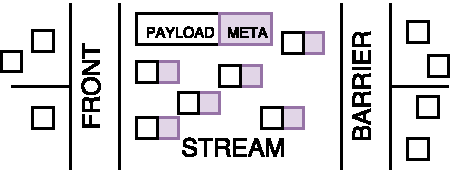
\includegraphics[width=0.48\textwidth]{pics/stream}
  \caption{The basic components of data flow}
  \label {stream}
\end{figure}

\subsection{Computational flow}

The stream between front and barrier is handled by a directed data flow graph. Each node of the graph represents a single operation, which can have multiple inputs and outputs. Edges indicate the order of these operations. Data items are processed one-by-one in a "streaming" manner. Figure~\ref{logical-graph-figure} shows the example of data flow graph.

Our model allows cycles in the graph while data flow graphs are commonly assumed to be acyclic (DAGs) 
~\cite{Zaharia:2016:ASU:3013530.2934664, Carbone:2017:SMA:3137765.3137777}. Moreover, as we show further, there are cases when cycles are required, e.g., for MapReduce-based algorithms. 

\subsection{Physical deployment and partitioning}
Data flow graph is distributed among computational units. Each unit runs a process called {\it worker}, and each of the workers executes complete data flow graph. An integer interval (hash range) is assigned to every worker. Intervals are not intersected and cover the range of 32-bit signed integer.

Each operation input has a user-provided hash function called {\it balancing function}. This function is applied to the payload of data items and determines partitioning before each operation. After that, the data items are sent to the worker, which is responsible for the associated hash range. Therefore, load balancing explicitly depends on the user-defined balancing functions. This allows the developer to determine optimal balancing which requires the knowledge of the payload distribution. The system optimizes the hash ranges assignment according to the processing statistics. Possible partitioning of this graph onto two nodes is shown in Figure~\ref{physical-graph-figure}. In this case, the first partition has the $[A, B)$ hash range and the second has the $[C, D)$. This example demonstrates the extreme case when the data item is shuffled between partitions after each operation.

\begin{figure}[htbp]
  \centering
  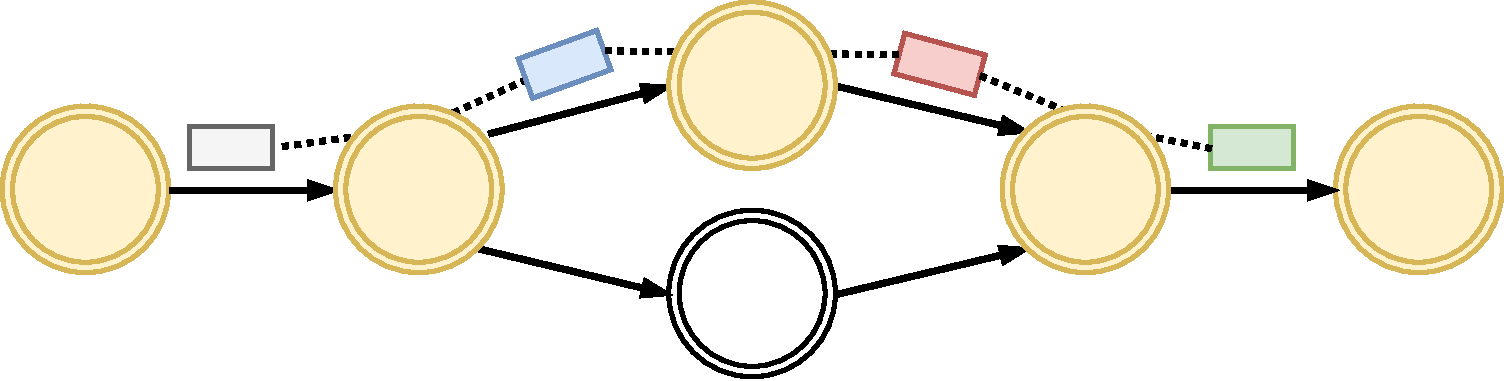
\includegraphics[width=0.48\textwidth]{pics/logical-graph}
  \caption{An example of the data flow graph}
  \label {logical-graph-figure}
\end{figure}

\begin{figure}[htbp]
  \centering
  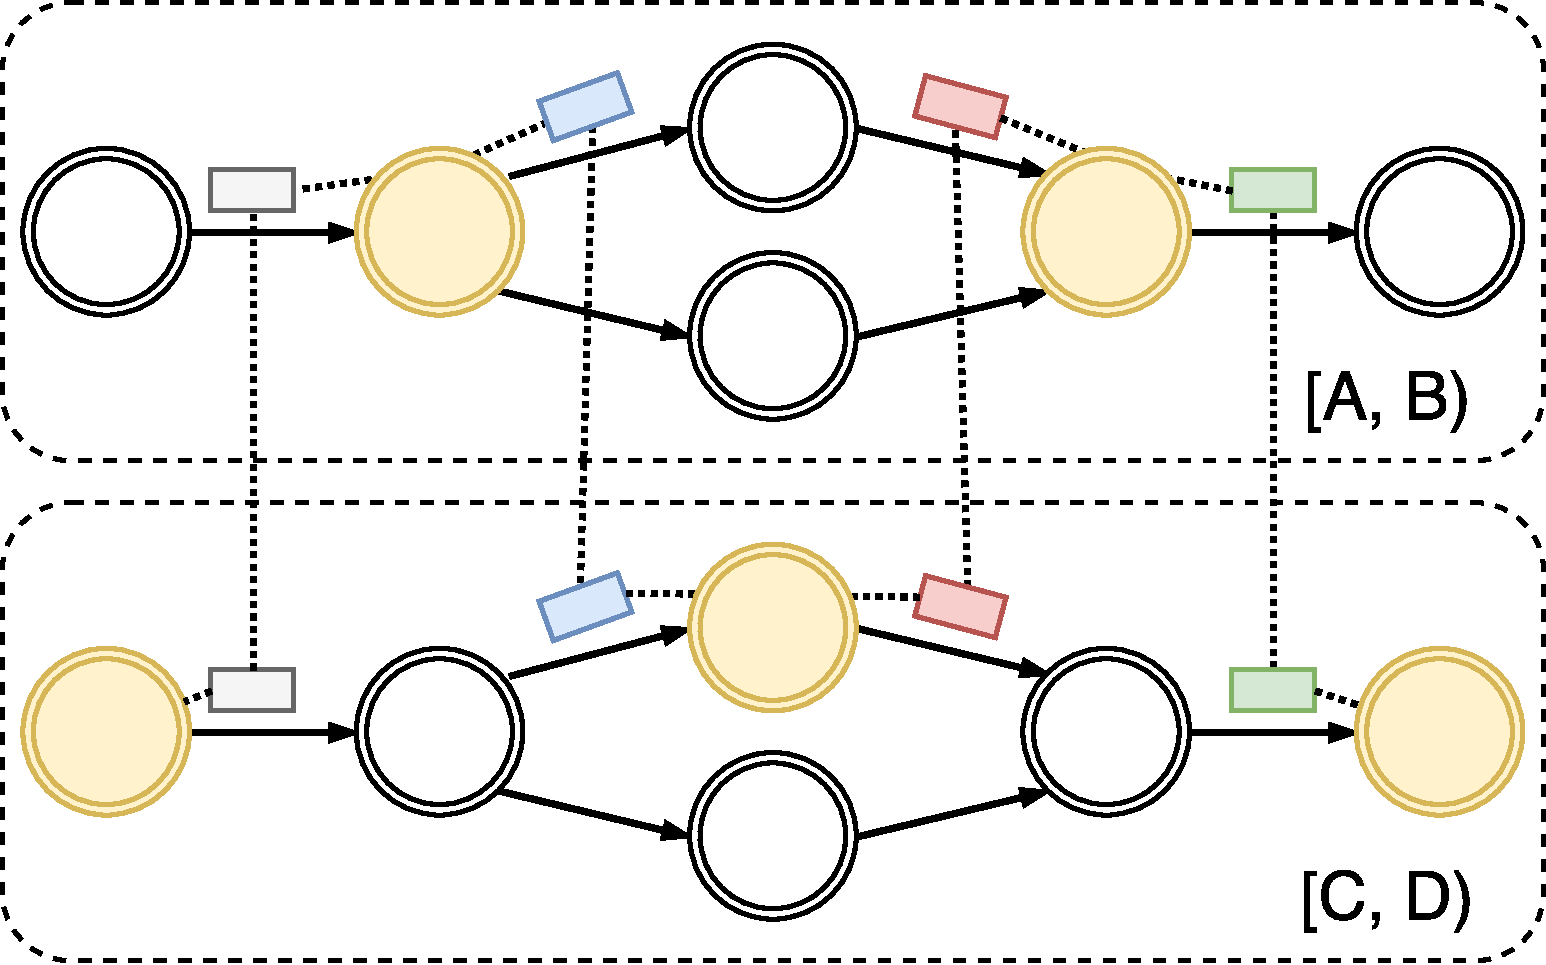
\includegraphics[width=0.48\textwidth]{pics/physical-graph}
  \caption{Possible partitioning of the data flow graph}
  \label {physical-graph-figure}
\end{figure}

\subsection{Ordering model}

We assume that there is a total order on data items. Ordering is preserved when an item is going through the operations. More precisely, the order of output items is the same as the order of corresponding input items. If more than one item is generated, they are inserted in output stream sequentially. Moreover, the output follows corresponding input but precedes the next item. Without diving into details, it should be noted that the order of items is maintained across different fronts.

The concept of ordering is shown in Figure~\ref{ordering}. Data item with payload $1'$ is the derivative of the item with payload $1$, according to operation $F$. The same is for items with payloads $2'$ and $2$. After union operation, the order between $1$ and $2$ is preserved. Furthermore, $1'$ follows $1$, and $2'$ follows $2$.  

\begin{figure}[htbp]
  \centering
  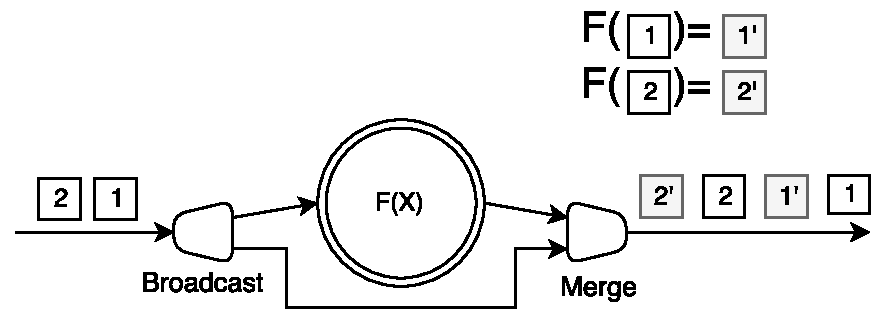
\includegraphics[width=0.5\textwidth]{pics/ordering}
  \caption{The concept of ordering model}
  \label {ordering}
\end{figure}

We assume that input items of the operations are strictly ordered.

\subsection{Operations}

The list of available operations includes:

{\bf Map} applies a user-defined function to the payload of an input item. This function returns a sequence of data items with transformed payloads. An output sequence can be empty.

{\bf Broadcast} replicates an input item to the specified number of operations.

{\bf Merge} operation is initialized with the specified number of input nodes. It sends all incoming data to the output.

{\bf Grouping} has a {\it window size} parameter. Grouping stores input items into distinct buckets by the value of the input balancing function applied to the payload. When the next item arrives at the grouping, it is appended to the corresponding bucket. Each time the grouping outputs window-sized {\it tuple item}, which consists of the most recent (in terms of the meta-information) items of this bucket. If the size of the bucket is less than the window, all items of the bucket are taken. Grouping is the only operation that has a state.

The following example illustrates the semantics of the operation. The grouping accepts items with payload represented as natural numbers: 1,2,3, etc. The hash function returns 1 if the number is even and 0 otherwise. If the window is set to 3, the output is:

\[(1), (2), (1|3), (2|4), (1|3|5), (2|4|6), (3|5|7), (4|6|8)...\]

There are two important properties of the grouping operation: the output tuple is identified by its last element, the results among items with different values of a hash function are independent.

\subsection{User-defined parameters}

A user can set up the following parameters:

\begin{enumerate}
  \item{Computational flow}
  \item{Balancing functions of the inputs}
  \item{Map functions}
  \item{Grouping windows}
\end{enumerate}

These parameters can produce more than one graph, which can yield equivalent results. Choosing among them is a performance optimization problem that relies on the system.
It is important to mention that there are no parameters for state-management. Therefore, business-logic is stateless. Nevertheless, the operations set is enough to implement any MapReduce transformation as shown in the next section.
